\documentclass[11pt,twocolumn]{article}
\title{Final Project: A Face Detector}
\author{Brendan Miller}
\date{March 12 2012}
\usepackage{multirow,amsmath}
\usepackage{graphicx}
\usepackage{fancyvrb}
\usepackage{color}
\usepackage{amsfonts}
\usepackage{hyperref}
\begin{document}
\twocolumn[
\begin{@twocolumnfalse}
\maketitle
\begin{abstract}
A face detector implemented via a simplified Viola Jones algorithm.
\end{abstract}
\end{@twocolumnfalse}
]

\section{Project Overview}

For this project I implemented an binary image classifier that detects
faces. This is based on the work of Paul Viola and Michael
Jones\cite{violajones2001}.

I extracted features from images by first generating what Viola and
Jones termed an integrated image. From the integrated image, I rapidly
computer a large number of real valued features, described more fully
in section \ref{sec:features}.

Given a large set of real valued features, I constructed a weak
learner by selecting a single feature and a threshold value that
partitioned example images into guessed face and non-face classes. This
weak learner is conceptually similar to a decision tree stump,
although the metric used to find the optimal feature and threshold is
different (see section \ref{sec:weaklearner}).

I combined weak learners using boosting (see section
\ref{sec:boosting}) in order to increase accuracy.

Finally, in the original Viola Jones paper, boosted classifiers were
combined in a cascade. The cascade was designed to reduce the
incidence of false positives, and to increase the performance of the
final classifier and possibly of the training phase. However, as stated
in my original project proposal, I have decided to descope the cascade
from this project in order to fit it into the time allotted.

Even without the cascade, I've managed to achieve very high accuracy,
upwards of 99\%\footnote{Note this is on a validation set selected
  from the images provided with this project.}, using a
boosted classifier over the features described in the original Viola
Jones paper.

\section{Feature Extraction}
\label{sec:features}

\begin{figure}
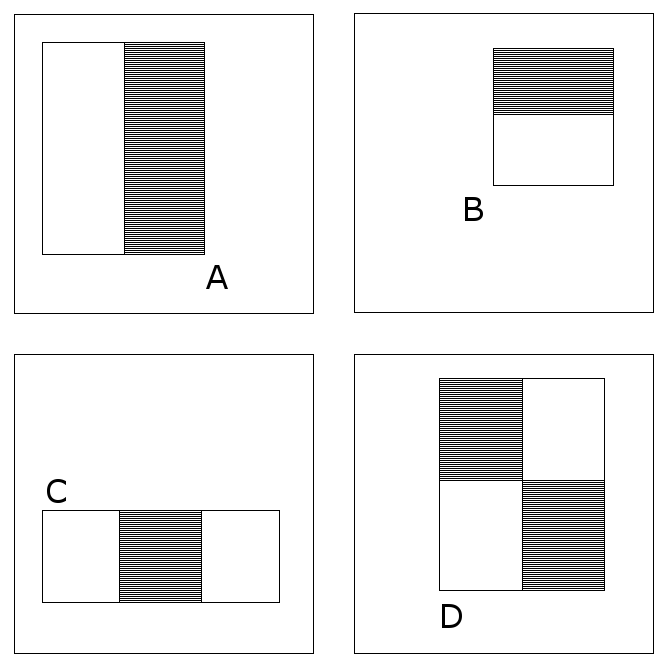
\includegraphics[width=60mm]{features.png}
\caption{Image features used to train the weak learner. Image from wikipedia.}
\label{fig:features}
\end{figure}

The underlying features used to train the weak classifier are
illustrated in figure \ref{fig:features}. These rectangular features
are computed by summing values of the pixels under the grayed out
section, and subtracting the sum of the pixels under the white section
to produce a real valued feature. For each feature type, every
possible scale and translation of the feature over the image is
computed.

These features and their rapid computation is probably the most
important innovation in Viola Jones. As discussed in the Viola Jones
paper\cite{violajones2001}, other detectors provide similar levels
of accuracy, but Viola Jones provides greatly improved performance and
is suitable for real time processing of image data.

To rapidly classify images, and also to provide more reasonable
training speeds, the features discussed in this paper can be quickly
computed by first creating an integral image. The integral image is of
the same dimension of the source image, but every element of the
integral image is the sum of all pixels above and to the left of that
coordinate in the source image.

From this integral image, the sum of a rectangular area can be
computer with only 4 array references, one to each corner of the
rectangle. A little algebra will similarly allow features A, B, C, and
D to be computed with a small number of references.

Even using the integrated image the performance of feature computation
can be a drag on the algorithm. When training on large datasets,
millions of features need to be computed. It is extremely important
that feature computation is fast. For this reason, after finding my
initial pure python implementation to be too slow, I rewrote the
feature extraction code in C++. This optimization made training about
5 times faster.

Another optimization that benefits the speed of training, but not of
classification, is to precompute all features and store them in main
memory. Originally I implemented my training stage this way, but found
that on large datasets the number of precomputed features was too
large to fit in main memory on a 32 bit machine.

For a 16 by 16 image, in my implementation there are 26944
features. Given 6000 training examples and 4 bytes per feature,
roughly 154 gigabytes of memory are necessary to precompute all the
features. Currently this is not practical.

\section{Feature Examples}

The most predictive features learned by the weak learner (see figure
\ref{fig:featureplot}) seem to focus around the eyes, which makes
sense as the eyes are probably the most uniform feature from face to
face. Comparatively, the mouth changes more, and may be covered by a
beard.

\begin{figure}
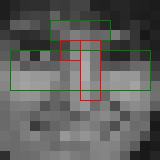
\includegraphics[width=60mm]{examples/features_plot.png}
\caption{Plot of 4 most predictive features on an image. Red indicates
  feature A, Green indicates feature B.}
\label{fig:featureplot}
\end{figure}

\section{Weak Learner}
\label{sec:weaklearner}

The weak learner used in the Viola Jones algorithm is very similar to
a stump decision tree classifier. The primary difference is that while
a stump classifier chooses a partition that maximizes weighted
information gain, the weak learner minimizes weighted
misclassification error.

\begin{align*}
  w_i = \mbox{weight of example $i$}\\
  h(x) = \mbox{weak learner classifier}\\
  \sum_i w_i |h(x_i) - y_i|
\end{align*}

This metric is important for performance reasons.

If for each feature we consider all thresholds mid way between the
unique values of the feature in sorted order, then for $K$ features and
$N$ examples there are $K (N - 1)$ feature threshold combinations.

For each feature assuming the examples are already sorted, the
threshold that minimizes weighted misclassification can be found in
linear time with respect to $N$ using a simple algorithm described in
Robust Real Time Face Detection\cite{violajones2004}. Finding the
threshold for each of $K$ features with minimal misclassification is
thus an $O(N K)$ operation\footnote{My current implementation
  technically runs in $O(K N \log(N))$ as I am sorting the examples
  over again for each round of boosting; however, profiling indicates
  that in practice this is not that big of a problem.}

Comparatively, calculating the information gain of an individual
partition is a linear time operation with respect to the number of
examples $N$. Since that operation needs to be performed $N - 1$ times
for each of the $K$ features, training a weak classifier using
information gain as a metric would take $O(K N^2)$ time.

\section{Boosted Classifier}
\label{sec:boosting}

The weak learners are combined in a fairly standard boosting algorithm
as described by Schapire\cite{schapire2001}. Since we covered boosting
in detail in the last assignment and the interesting aspects of the
Viola Jones technique are in the weak learner and the cascade, I will
omit a detailed discussion of boosting.

Taking $M$ rounds of boosting into account and the total complexity of
the training phase is $O(N K M)$.

\section{Experimental Results}

My training data\cite{trainingdata} is provided with my project and
consists of 3000 images of faces and 10000 images of non-faces. All
are 16 X 16 grayscale images.

Using 50 rounds of boosting and 5000 randomly selected training
images, I produced a classifier\footnote{This classifier is serialized
  as JSON in the file large\_classifier.json.}  that accurately
classified faces over a held out validation set of 1000 images with
0.9\% error. It produced 5 false positives and 4 false negatives.

This classifier is relatively rapid. In one test once the integrated
images had been generated, classification of 6000 images took place in
1180 milliseconds using the C++ backend\footnote{By comparison the
  python backend took 9615 milliseconds.}. Thus it takes about 0.2
milliseconds to classify an individual image.

\begin{figure}
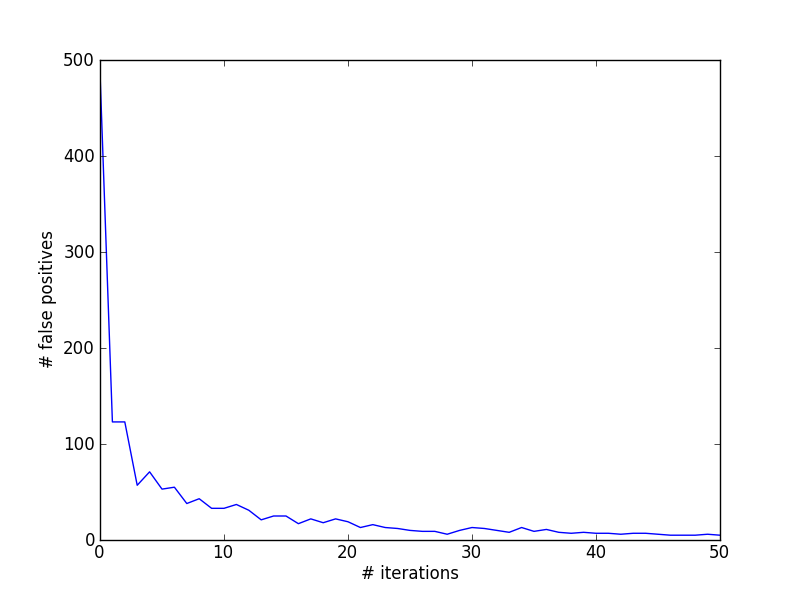
\includegraphics[width=70mm]{false_positives.png}
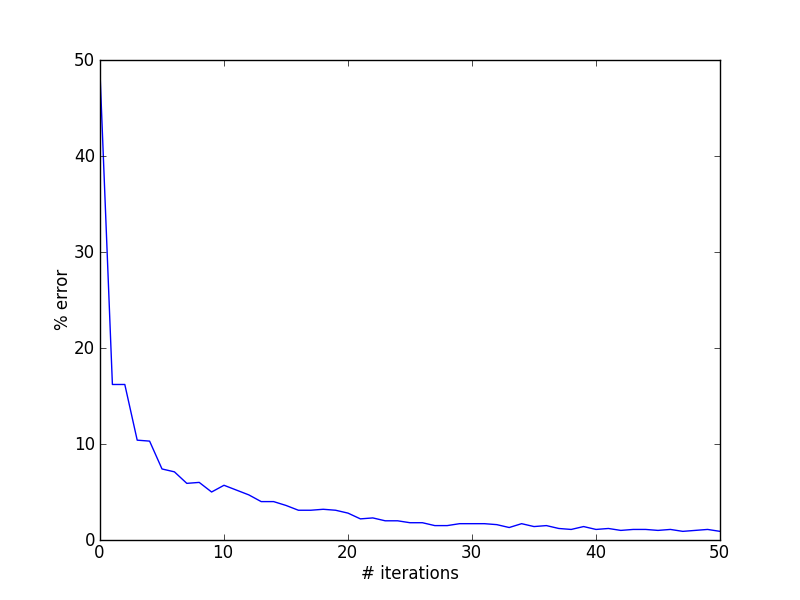
\includegraphics[width=70mm]{pct_err.png}
\caption{Percent error over 1000 held out validation images given
  rounds of boosting. Classifier trained from 5000 images.}
\label{fig:bootingiter}
\end{figure}



Thus even without the cascade described in the Viola Jones paper,
it's possible to build a very good face classifier of whole
images. However, in order to detect faces within a larger image, it's
necessary to run the classifier many thousands of times at different
locations and scales. In this scenario, 4 false positives out of 1000
is actually too high. See figure \ref{fig:searchfalsepositives}.

\begin{figure}
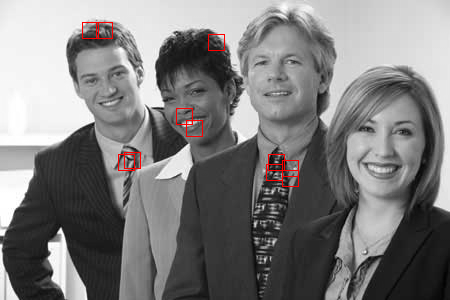
\includegraphics[width=60mm]{examples/search_out.png}
\caption{False positives within a larger image.}
\label{fig:searchfalsepositives}
\end{figure}

Adding the cascade in the original Viola Jones paper would probably
resolve this issue, but that feature was scoped out of this project at
proposal time due to the time constraints of the project.

\section{Future Directions}

I'd like to experiment with measures to further reduce false
positives. The obvious choice would be to add in the cascade. However,
my suspicion is that other perhaps simpler mechanisms could reduce
false positives. My suspicion is that the Viola Jones cascade in
practice mainly serves as an elaborate biasing mechanism, encoding the
knowledge that non-faces are far more common than faces into the
classifier.

I think it should be possible to either introduce a simpler biasing
mechanism into adaboost, or to encode the knowledge into the data by
adjusting the ratio of faces to non-faces in the training data.

Another future direction would be to speed up the training process by
either introducing multiple threads, or spreading the work across a
map reduce cluster.

\begin{thebibliography}{9}

\bibitem{violajones2001}
  Paul Viola, Michael Jones\\
  Rapid Object Detection using a Boosted Cascade of Simple Features\\
  \url{http://research.microsoft.com/en-us/um/people/viola/Pubs/Detect/violaJones_CVPR2001.pdf}

\bibitem{violajones2004}
  Paul Viola, Michael Jones\\
  Robust Real Time Face Detection\\
  \url{http://www.vision.caltech.edu/html-files/EE148-2005-Spring/pprs/viola04ijcv.pdf}

\bibitem{schapire2001}
  Robert E. Schapire\\
  The Boosting Approach to Machine Learning: An Overview\\
  \url{http://www.cs.princeton.edu/~schapire/uncompress-papers.cgi/msri.ps}

\bibitem{trainingdata}
  Training data used for my project\\
  \url{http://www.stat.ucla.edu/~yuille/courses/Stat231-Fall08/}

\end{thebibliography}



\end{document}